\documentclass[a4paper,11pt]{article}

\usepackage{amsmath,amssymb}
\usepackage{graphicx}
\usepackage[percent]{overpic}
\usepackage{tikz}
\usepackage{circuitikz}
\usetikzlibrary{shapes.misc}

\usepackage{fancyvrb}

\usepackage[labelfont=bf]{caption}
\captionsetup{labelfont=bf}

\ctikzset{bipoles/length=20pt}  % Size of schematic components

\usetikzlibrary{decorations.markings}
\tikzset{-dot-/.style={decoration={
    markings,
    mark=at position #1 with {\fill circle (2pt);}},postaction={decorate}}
}
\tikzset{-ddot-/.style={decoration={
    markings,
    mark=at position #1 with {\draw[dashed,thick] circle (2pt);}},postaction={decorate}}
}

\usepackage{abstract}
\renewcommand{\abstractname}{}
\renewcommand{\absnamepos}{empty}

% Render inline citations in superscript.
\let\oldcite\cite
\renewcommand{\cite}[1]{\textsuperscript{\oldcite{#1}}}

\title{Modelling single-electron transport\\through nanocrystals}
\author{Candidate: Nicolas Bricknell\\Supervisor: Prof.~Chris Ford}

\begin{document}
    \maketitle
    \begin{abstract}
        \noindent A model of transport through a quantum dot is introduced, based on rate equations, constant interaction and Fermi's golden rule. The model is implemented numerically using both eigenvalue and \textsc{ode} methods. The faster \textsc{ode} method is used to investigate and account for current characteristics in two main regimes: quantum mechanical-dominated and electrostatically-dominated. The effects of spin degeneracy, source-drain asymmetry and singularities in lead densities-of-states are studied, and the results found to be largely consistent with experimental observations. The model is applied tentatively to the case of n-doped semiconducting leads. Finally, possible ways to improve the implementation are suggested, including relaxing the assumption of constant interaction and incorporating electronic relaxation.
    \end{abstract}

    \newpage
    \tableofcontents


    \newpage
    \section{Introduction}
    The past 25 years has seen growing interest in single-electron effects in nanocrystals contacted by current-bearing electrodes. Coulomb blockade is a well-understood phenomenon in which the electrostatic energy required to add an electron to a nanocrystal exceeds the energy available in the electrodes, so that no current can flow through. Varying the electrostatic energy requirement by means of a gate voltage, to optionally lift the blockade, presents a way to realise a so-called single-electron transistor (\textsc{set}).

    Separately from electrostatic considerations, a sufficiently small nanocrystal has a discrete energy spectrum, and may be called a quantum dot. The interplay of quantum-mechanical energies with the aforementioned charging energy results in complex current characteristics for transport through the nanocrystal. At the same time, the discreteness of available energy levels in the dot presents a conceptually simple way to model this transport via a set of rate equations. The present work is based on a computational implementation of those rate equations and an exploration of their consequences.

    Quantum Coulomb blockade can be used to infer the energy levels of `artificial-atom'-like nanocrystals\cite{Banin-1999}, and single-electron devices of the type discussed in this report could form a basis for high-density data storage systems\cite{Likharev-1999} or be used in spin-based quantum computation\cite{Zutic-2004}.


    \section{Theory}

    A nanocrystal can be thought of as a potential well, separated by tunnel barriers from source and drain electrodes (fig.~\ref{fig:Setup_schematics}). The source and drain electrodes (`leads') usually have a continuous energy spectrum. Energy conservation and Fermi statistics dictate when a given tunnelling process is possible.

    \begin{figure}[h!]
    \begin{center}
        \makebox[\textwidth]{
            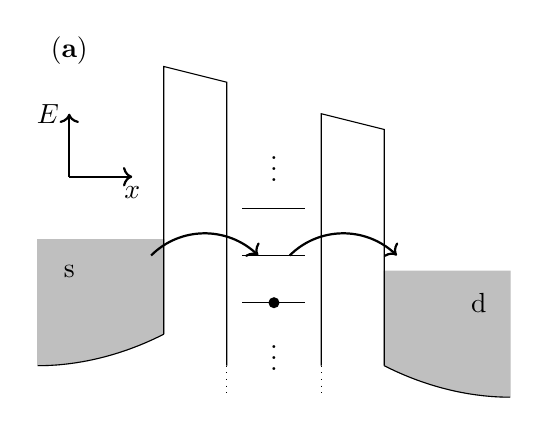
\begin{tikzpicture}[scale=0.4]
                \filldraw[color=lightgray] (0,-2) parabola (4,-1) -- (4,2) -- (0,2) -- cycle;
                \draw (0,-2) parabola (4,-1);
                \filldraw[color=lightgray] (15,-3) parabola (11,-2) -- (11,1) -- (15,1) -- cycle;
                \draw (15,-3) parabola (11,-2);
                \draw (4,-1) -- (4, 7.5) -- (6,7) -- (6,-2);
                \draw[dotted] (6,-2) -- (6,-3);
                \draw[dotted] (9,-2) -- (9,-3);
                \draw (9,-2) -- (9,6) -- (11,5.5) -- (11,-2);
                
                \draw[->,thick] (3.6,1.5) to [bend left=45] (7,1.5);
                \draw[->,thick] (8.0,1.5) to [bend left=45] (11.4,1.5);
                
                % Dot orbitals
                \draw (6.5,1.5) -- (8.5,1.5);
                
                \draw (6.5,3) -- (8.5,3);
                \draw[-dot-=0.5] (6.5,0) -- (8.5,0);
                
                \node at (1,8) {(\textbf{a})};
                \node at (1,1) {s};
                \node at (14,0) {d};
                
                \node at (7.5,-1.5) {$\vdots$};
                \node at (7.5,4.5) {$\vdots$};
                
                \draw[thick,->] (1,4) -- (3,4) node[anchor=north] {$x$};
                \draw[thick,->] (1,4) -- (1,6) node[anchor=east] {$E$};
            \end{tikzpicture}
            \hspace{30pt}
            \begin{tikzpicture}[scale=0.5]
                \draw
                  (0,0) [-o] to (4.2,0) node[anchor=west] {$V_\mathrm{sd}$} node[anchor=north] {$+$};
                \draw
                  (10,0) [-o] to (5.8,0) node[anchor=north] {$-$};
                \draw
                  (10,0) to (10,4);
                \draw
                  (5,8)
                  to [C, l_=$C_\mathrm{g}$] (5,4) to (6,4) to (6,5)
                  to [R, l_=$R_\mathrm{d}$] (9,5) to (9,4) to (10,4);
                \draw
                  (6,4) to (6,2.5)
                  to [C, l_=$C_\mathrm{d}$] (9,2.5) to (9,4);
                \draw
                  (0,0) to (0,4) to (1,4) to (1,5)
                  to [R, l_=$R_\mathrm{s}$] (4,5) to (4,4) to (5,4);
                \draw
                  (1,4) to (1,2.5)
                  to [C, l_=$C_\mathrm{s}$] (4,2.5) to (4,4);
                \draw (5,8) [-o] to (6,8) node[anchor=west] {$V_\mathrm{g}$};
                
                \node at (0,8) {(\textbf{b})};
            \end{tikzpicture}
        }
        \caption{Model of a nanocrystal between electrodes. (\textbf{a}) illustrates how current only flows through a dot level if its electrochemical potential lies between source and drain Fermi levels. (\textbf{b}) is an approximate circuit diagram for the nanocrystal lying between source and drain barriers and capacitively coupled to a gate voltage (after Kouwenhoven~\textit{et~al.}\cite{Kouwenhoven-1991}).}
        \label{fig:Setup_schematics}
    \end{center}
    \end{figure}

    The nanocrystal may be capacitively coupled to a gate voltage as shown in fig.~\ref{fig:Setup_schematics}(b). Increasing the gate voltage lowers the electrochemical potential of all electronic states in the nanocrystal. In addition, the tunnel barriers to source and drain have some capacitance, so that the energies in the dot are also offset by a `lever-arm' voltage which `leaks' over the tunnel barriers when a bias $V_\mathrm{sd}$ is applied, depending on the relative values of source and drain capacitances $C_\mathrm{s}$ and $C_\mathrm{d}$.

    Each dot level has an electrochemical potential which depends on the arrangement of other electrons in the dot. An electrochemical potential is simply a measure of the energy required for a process to occur which also incorporates the effect of electrostatics. If no dot level has an electrochemical potential lying between the source and drain Fermi levels, then no current can flow and the nanocrystal is said to undergo blockade.

    \subsection{Model of quantum Coulomb blockade}
    In order to numerically model transport, I use a number of assumptions, some of which are more deeply tied to the computational scheme than others. The four principle approximations are adopted from the work of Beenakker\cite{Beenakker-1991}:
    \begin{itemize}
        \item I use rate equations which presuppose that electrons pass through tunnel barriers independently and directly from an occupied state to an empty state.
        \item I assume that the rate of transport through a single tunnel barrier is described accurately by Fermi's golden rule.
        \item I use the model of constant interaction. This is the assumption that there is no preferential Coulombic interaction between electrons in any pair of dot levels; the potential of each level is simply offset by an amount determined by the total charge on the dot.
        \item As a corollary to constant interaction, the total capacitance of the dot is independent of its total occupancy (even when the dot is singly occupied, for instance).
    \end{itemize}

    Throughout this report, I use the following meaning: an \textit{occupation configuration} is the set of occupation numbers (each either $0$ or $1$) for the energy levels in a quantum dot. For instance, if a dot's lowest three energy levels\footnote{``Lowest energy level'' could either refer to the true lowest-energy orbital, or to the lowest unoccupied molecular orbital (\textsc{lumo}) in the case of a semiconductor dot.} are occupied, then its occupation configuration is $\{1,1,1,0,0,\dots\}$.

    As electrons tunnel in and out of the dot via the tunnel barriers to leads, they alter the dot's occupation configuration. This gives rise to flux between different configurations, so that each has a \textit{weight}. A configuration's weight is the fraction of time the dot spends in that configuration. I call the set of all weights (one for each configuration) the \textit{weights vector}.

    \subsubsection{Beenakker's rate equations}
    To quantify the flux between occupation configurations, I follow rate equations from Beenakker\cite{Beenakker-1991}, cast into matrix form and generalised to account for an arbitrarily varying density of states in the leads. To illustrate, consider a two-level system. $n_l$ represents the occupation number of the $l$th level in the quantum dot, taking value 0 or 1. There are four possible configurations:
    \begin{equation}\label{eqn:Two-level_configurations}\begin{aligned}
        \{n_l\}_\alpha = \{0,0\}, \\
        \{n_l\}_\beta  = \{1,0\}, \\
        \{n_l\}_\gamma = \{0,1\}, \\
        \{n_l\}_\delta = \{1,1\}.
    \end{aligned}\end{equation}
    Labelling the weight of the $\eta$th configuration as $w_\eta$, the flux between the different configurations $\{n_l\}$ is given by
    \begin{equation}\label{eqn:Rate_matrix}\resizebox{.93\hsize}{!}{$
        \frac{\mathrm{d}}{\mathrm{d} t} \left( \begin{matrix} w_\alpha \\ w_\beta \\ w_\gamma \\ w_\delta \end{matrix} \right)
      = \left( \begin{matrix}
                   -\left(i_{0|\alpha} + i_{1|\alpha}\right)
                 &  o_{0|\beta}
                 &  o_{1|\gamma}
                 &  0 \\
                    i_{0|\alpha}
                 & -\left(o_{0|\beta} + i_{1|\beta}\right)
                 &  0
                 &  o_{1|\delta} \\
                    i_{1|\alpha}
                 &  0
                 & -\left(i_{0|\gamma} + o_{1|\gamma}\right)
                 &  o_{0|\delta} \\
                    0
                 &  i_{1|\beta}
                 &  i_{0|\gamma}
                 & -\left(o_{0|\delta} + o_{1|\delta}\right)
               \end{matrix} \right)
        \left( \begin{matrix} w_\alpha \\ w_\beta \\ w_\gamma \\ w_\delta \end{matrix} \right).
    $}\end{equation}
    Here $i_{l|\eta}$ represents the instantaneous rate of tunnelling in to the $l$th dot level, given a starting configuration $\eta$. This quantity partitions into contributions from the two current-bearing electrodes, source and drain:
    \begin{equation}\label{eqn:Partition}
        i_{l|\eta} = i_{l|\eta}^\mathrm{s} + i_{l|\eta}^\mathrm{d}.
    \end{equation}
    The same partitioning applies to the rate of tunnelling out, $o_{l|\eta}$.

    In writing down equation~\ref{eqn:Rate_matrix} we neglect simultaneous tunnelling events involving two dot levels, which would contribute in this case to the anti-diagonal matrix elements. Furthermore, we neglect intra-dot radiative decay (`relaxation'), which would contribute to the $(2,3)$ matrix element in equation~\ref{eqn:Rate_matrix}.

    Matrix equation~\ref{eqn:Rate_matrix} generalises straightforwardly to an $N$-level system. Its steady-state solution (i.e.\ weights vector) can be found either by a linear algebra approach, or by direct evolution of the weights with time (discussed in Section~\ref{sec:Implementation}). The total current through the dot at any particular time is
    \begin{equation}\label{eqn:Current}
        I{(t)} = -e \sum\limits_\eta w_\eta{(t)}
                   \sum\limits_l
                       \begin{cases}
                           o_{l|\eta}^\mathrm{drain} - o_{l|\eta}^\mathrm{source}, & n_{l,\eta} = 1 \\
                           i_{l|\eta}^\mathrm{source} - i_{l|\eta}^\mathrm{drain}, & n_{l,\eta} = 0
                       \end{cases}
    \end{equation}
    where $\eta$ runs over all configurations $\{\alpha, \beta,\dots\}$ and $l$ runs over all dot levels.

    \subsubsection{Electrochemical potentials}
    In order to reason about tunnelling in and out of the dot, we must know the electrochemical potentials of the available levels in the dot. For this quantity, I use the following symbols. For $\mu^+_{l|\eta}$ read ``the energy at which an electron can tunnel \textit{in} to the $l$th dot level, given a \textit{starting} configuration $\eta$''. This is distinct from $\mu^-_{l|\eta}$, the energy at which an electron can tunnel \textit{out} of the $l$th dot level given a starting configuration $\eta$. Only one of the quantities $\mu^\pm_{l|\eta}$ is well-defined for a given $l,\eta$ pair. For instance, $\mu^-_{l|\eta}$ is meaningless if level $l$ is not already occupied in the $\eta$th configuration.

    In the model of constant interaction, the total energy associated with the nanocrystal, in any particular configuration, is given by the sum of the single-particle energies of its occupied levels, plus an electrostatic energy $Q^2/2C_\mathrm{tot}$. From this starting point, it can be shown (appendix~\ref{sec:Chemical_potential}) that the electrochemical potentials as defined above are given by
    \begin{equation}\label{eqn:Chemical_potential}
        \mu^\pm_{l|\eta} = E_l + \frac{e}{\sum_i C_i}\left[\left(N_\eta \pm \frac{1}{2}\right)e - \sum_i C_i V_i\right],
    \end{equation}
    where $N_\eta$ is the sum of the occupation numbers in configuration $\eta$, and $E_l$ is the single-particle energy of the $l$th level. $i$ runs over the source, drain and gate electrodes (fig~\ref{fig:Setup_schematics}(b)), so the above expression naturally incorporates the `lever-arm' voltage on the dot, as well as the capacitive coupling to the gate voltage. The right-hand side contains contributions from the single-particle energy and the classical charging energy.

    If the single-particle energies vanished, potentials for successive electron additions would be separated by $\Delta \mu = e^2/\sum_i C_i \equiv e^2/C_\mathrm{tot}$. For this reason, the quantity $e^2/C_\mathrm{tot}$ is called the charging energy. The principal diamonds in fig.~\ref{fig:Degeneracy}(a) (regions in which the nanocrystal exhibits Coulomb blockade) have a height proportional to this charging energy. Moving up through successive diamonds, we can picture the dot filling up with electrons as the gate voltage is increased. If the single-particle energies do not vanish, then the energy required to add successive electrons ($\Delta \mu$) is increased by the single-particle energy spacing $\left(E_{l+1} - E_l\right)$, as demonstrated by fig.~\ref{fig:Degeneracy}(b).

    \begin{figure}[p]
    \begin{center}
        \makebox[\textwidth]{\begin{overpic}[scale=0.4]{img/degenerate_case.pdf}\put(5,73){(\textbf{a})}\end{overpic}\begin{overpic}[scale=0.4]{img/broken_degeneracy.pdf}\put(5,73){(\textbf{b})}\end{overpic}}
        \caption{Conductance as a function of source-drain bias and gate voltage, showing conventional Coulomb blockade diamonds (calculated via rate equations). Dark shades represent large values of source-drain conductance; white represents zero conductance. (\textbf{a})~shows conductance in the absence of quantum-mechanical energy contributions. (\textbf{b})~illustrates two effects of the single-particle energy: the size of the blockade diamonds is increased, and the conductance shows more peaks outside the blockade diamonds, corresponding to the excitation spectrum.}
        \label{fig:Degeneracy}
    \end{center}
    \end{figure}

    %For \textsc{homo} instead of \textsc{lumo} tunnelling, flip figure~\ref{fig:Degeneracy} upside down. Fig.~\ref{fig:Degeneracy}(a) not valid outside Coulomb diamonds -- would need to use orthodox theory calculations.

    \begin{figure}[p]
    \begin{center}
        \makebox[\textwidth]{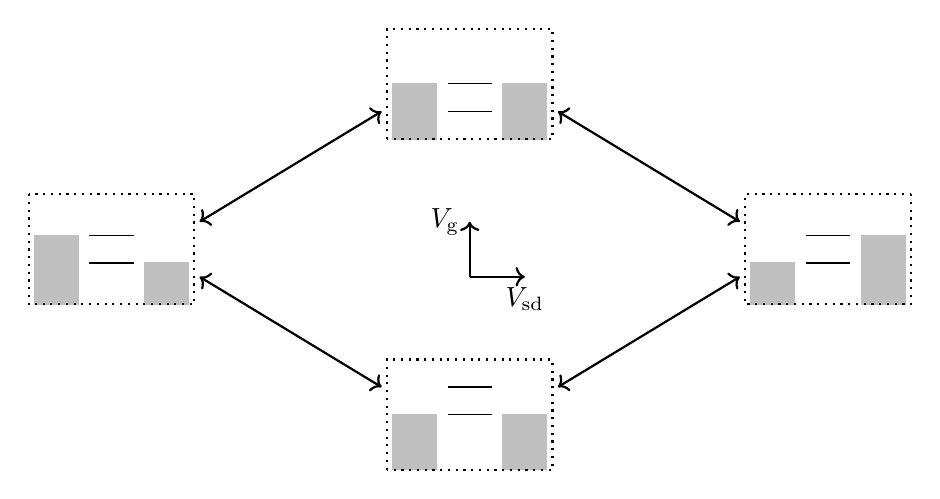
\begin{tikzpicture}[scale=0.7]
        % Diamond
        \draw[->,thick] (3.25,1) -- (4.9,2);
        \draw[->,thick] (3.25,1) -- (1.6,0);
        
        \draw[->,thick] (3.25,4) -- (4.9,3);
        \draw[->,thick] (3.25,4) -- (1.6,5);
        
        \draw[->,thick] (-3.25,1) -- (-4.9,2);
        \draw[->,thick] (-3.25,1) -- (-1.6,0);
        
        \draw[->,thick] (-3.25,4) -- (-4.9,3);
        \draw[->,thick] (-3.25,4) -- (-1.6,5);
        
        % Axes
        \draw[thick,->] (0,2) -- (1,2) node[anchor=north] {$V_\mathrm{sd}$};
        \draw[thick,->] (0,2) -- (0,3) node[anchor=east] {$V_\mathrm{g}$};
        
        % Bottom diagram
        \filldraw[lightgray] (-1.4,-0.5) -- (-0.6,-0.5) -- (-0.6,-1.5) -- (-1.4,-1.5) -- cycle;  % Source
        \filldraw[lightgray] (1.4,-0.5) -- (0.6,-0.5) -- (0.6,-1.5) -- (1.4,-1.5) -- cycle;  % Drain
        \draw (-0.4,0) -- (0.4,0);  % Upper
        \draw (-0.4,-0.5) -- (0.4,-0.5);  % Lower
        \draw[dotted,thick] (-1.5,-1.5) -- (-1.5,0.5) -- (1.5,0.5) -- (1.5,-1.5) -- cycle;  % Box
        
        % Top diagram
        \filldraw[lightgray] (-0.6,5.5) -- (-0.6,4.5) -- (-1.4,4.5) -- (-1.4,5.5) -- cycle;  % Source
        \filldraw[lightgray] (0.6,5.5) -- (0.6,4.5) -- (1.4,4.5) -- (1.4,5.5) -- cycle;  % Drain
        \draw (-0.4,5.5) -- (0.4,5.5);  % Upper
        \draw (-0.4,5) -- (0.4,5);  % Lower
        \draw[dotted,thick] (-1.5,4.5) -- (-1.5,6.5) -- (1.5,6.5) -- (1.5,4.5) -- cycle;  % Box
        
        % Left diagram
        \filldraw[lightgray] (-7.9,1.5) -- (-7.1,1.5) -- (-7.1,2.75) -- (-7.9,2.75) -- cycle;  % Source
        \filldraw[lightgray] (-5.9,1.5) -- (-5.1,1.5) -- (-5.1,2.25) -- (-5.9,2.25) -- cycle;  % Drain
        \draw (-6.9,2.75) -- (-6.1,2.75);  % Upper
        \draw (-6.9,2.25) -- (-6.1,2.25);  % Lower
        \draw[dotted,thick] (-8,3.5) -- (-8,1.5) -- (-5,1.5) -- (-5,3.5) -- cycle;  % Box
        
        % Right diagram
        \filldraw[lightgray] (7.9,1.5) -- (7.1,1.5) -- (7.1,2.75) -- (7.9,2.75) -- cycle;  % Source
        \filldraw[lightgray] (5.9,1.5) -- (5.1,1.5) -- (5.1,2.25) -- (5.9,2.25) -- cycle;  % Drain
        \draw (6.9,2.75) -- (6.1,2.75);  % Upper
        \draw (6.9,2.25) -- (6.1,2.25);  % Lower
        \draw[dotted,thick] (8,3.5) -- (8,1.5) -- (5,1.5) -- (5,3.5) -- cycle;  % Box
        \end{tikzpicture}}
        \caption{Meaning of movements in the $\left(V_\mathrm{sd},V_\mathrm{g}\right)$ plane, in the context of a blockade diamond. Each inset is an energy diagram for the dot levels, between source and drain leads, at one of the corners of a blockade diamond. Along~$\nearrow$~and~$\swarrow$~paths, dot levels move in sync with the source Fermi level. Along~$\nwarrow$~and~$\searrow$~paths they move with the drain Fermi level. Conductance peaks occur when source or drain Fermi level moves past an electrochemical potential. This figure neglects charging energies for clarity.}
        \label{fig:Directions}
    \end{center}
    \end{figure}

    \subsubsection{Fermi's golden rule}
    In the limit of small overlap between the dot orbitals and lead wavefunctions, we can approximate the tunnelling rates from eqn.~\ref{eqn:Partition} using Fermi's golden rule:
    \begin{equation}\label{eqn:Tunnel_rate_in}
        i_{l|\eta}^\mathrm{s,d} = \Gamma^\mathrm{s,d}_l \times f{\left(\mu^+_{l|\eta} \mp \frac{\left(-e\right)V_\mathrm{sd}}{2}\right)} \times g^\mathrm{s,d}{\left(\mu^+_{l|\eta} \mp \frac{\left(-e\right)V_\mathrm{sd}}{2}\right)},
    \end{equation}
    where the minus signs correspond to $\mathrm{s}$, and plus to $\mathrm{d}$. Here $\Gamma^\mathrm{s,d}_l$ is the tunnelling width from source/drain lead to $l$th dot level, $f$ is the Fermi-Dirac function and $g^\mathrm{s,d}$ is the source/drain lead density of states. For tunnelling out of the dot we have
    \begin{equation}\label{eqn:Tunnel_rate_out}
        o_{l|\eta}^\mathrm{s,d} = \Gamma^\mathrm{s,d}_l \times \left[1 - f{\left(\mu^-_{l|\eta} \mp \frac{\left(-e\right)V_\mathrm{sd}}{2}\right)}\right] \times g^\mathrm{s,d}{\left(\mu^-_{l|\eta} \mp \frac{\left(-e\right)V_\mathrm{sd}}{2}\right)} .
    \end{equation}

    In principle, the tunnelling widths also depend on the electrochemical potentials, but for the purposes of this report I have neglected this fact.

    \subsection{Electrochemical potential diagrams}
    Even within the constant interaction model (eqn.~\ref{eqn:Chemical_potential}), it is nevertheless true that each configuration has a different set of energies at which electrons may tunnel in and out (in general). I call each such set of energies a ``$\mu$~spectrum''.

    In order to represent these $\mu$ spectra and thereby elucidate the effect of charging on transport, I use a non-standard type of energy diagram. Each such diagram corresponds to a particular dot configuration, with the following rules:
    \begin{itemize}
        \item Each dot level is shown by a horizontal line.
        \item If a level is occupied, it is shown with a small overlayed circle.
        \item If a level is not occupied, its height illustrates the gross energy required to occupy it (i.e.\ the sum of single-particle and Coulomb energies). This is the energy level at which an electron may tunnel in from an electrode.
        \item If a level is occupied, its height illustrates the gross energy liberated upon vacating it. This is the energy level at which the electron may tunnel out to an electrode.
    \end{itemize}
    This type of diagram differs from conventional energy diagrams by the fact that it \textit{simultaneously} shows addition energies~($\mu^+$) and removal energies~($\mu^-$). Fig.~\ref{fig:Sequential_diagrams} exemplifies.

    In addition, it is sometimes useful to show two configurations (e.g.\ before and after a tunnelling event), and therefore two $\mu$~spectra, on the same diagram. When this is done, one of the spectra is shown with dashed lines. Fig.~\ref{fig:Combined_diagram}(a) is an example.

    \begin{figure}[p]
    \begin{center}
        \makebox[\textwidth]{
            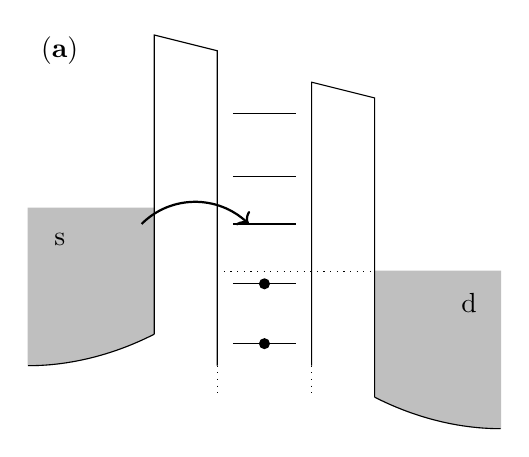
\begin{tikzpicture}[scale=0.4]
                \filldraw[color=lightgray] (0,-3) parabola (4,-2) -- (4,2) -- (0,2) -- cycle;
                \draw (0,-3) parabola (4,-2);
                \filldraw[color=lightgray] (15,-5) parabola (11,-4) -- (11,0) -- (15,0) -- cycle;
                \draw (15,-5) parabola (11,-4);
                
                \draw (4,-2) -- (4, 7.5) -- (6,7) -- (6,-3);
                \draw[dotted] (6,-3) -- (6,-4);
                
                \draw[dotted] (9,-3) -- (9,-4);
                \draw (9,-3) -- (9,6) -- (11,5.5) -- (11,-4);
                
                \draw[->,thick] (3.6,1.5) to [bend left=45] (7,1.5);
                
                % Dot orbitals
                \draw (6.5,5) -- (8.5,5);
                
                \draw (6.5,3) -- (8.5,3);
                
                \draw (6.5,1.5) -- (8.5,1.5);
                
                \draw[-dot-=0.5] (6.5,-0.4) -- (8.5,-0.4);
                
                \draw[-dot-=0.5] (6.5,-2.3) -- (8.5,-2.3);
                
                % Labels
                \node at (1,1) {s};
                \node at (14,-1) {d};
                
                \draw[dotted] (6,0) -- (11,0);
                
                \node at (1,7) {(\textbf{a})};
            \end{tikzpicture}\begin{tikzpicture}[scale=0.3]
                \draw[white] (-1,0) -- (11,0);
                \draw[->,thick] (1,8) to node[midway,above] {followed by}  (9,8);
                \end{tikzpicture}
            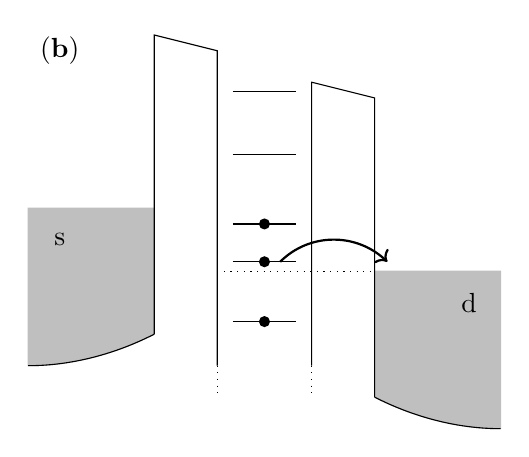
\begin{tikzpicture}[scale=0.4]
                \filldraw[color=lightgray] (0,-3) parabola (4,-2) -- (4,2) -- (0,2) -- cycle;
                \draw (0,-3) parabola (4,-2);
                \filldraw[color=lightgray] (15,-5) parabola (11,-4) -- (11,0) -- (15,0) -- cycle;
                \draw (15,-5) parabola (11,-4);
                
                \draw (4,-2) -- (4, 7.5) -- (6,7) -- (6,-3);
                \draw[dotted] (6,-3) -- (6,-4);
                
                \draw[dotted] (9,-3) -- (9,-4);
                \draw (9,-3) -- (9,6) -- (11,5.5) -- (11,-4);
                
                \draw[->,thick] (8.0,0.3) to [bend left=45] (11.4,0.3);
                
                % Dot orbitals
                \draw (6.5,5.7) -- (8.5,5.7);
                
                \draw (6.5,3.7) -- (8.5,3.7);
                
                \draw[-dot-=0.5] (6.5,1.5) -- (8.5,1.5);
                
                \draw[-dot-=0.5] (6.5,0.3) -- (8.5,0.3);
                
                \draw[-dot-=0.5] (6.5,-1.6) -- (8.5,-1.6);
                
                % Labels
                \node at (1,1) {s};
                \node at (14,-1) {d};
                
                \draw[dotted] (6,0) -- (11,0);
                
                \node at (1,7) {(\textbf{b})};
            \end{tikzpicture}
        }
        \caption{Possible impact of charging on transport. In (\textbf{a}) an electron tunnels from source lead to the third dot level. This raises the electrochemical potential of all other levels by $e^2/C_\mathrm{tot}$. (The potential of the third level is not raised because its value already included the charging energy, and its electron could now tunnel out at the same energy as it came in.) The new, higher energies are shown in (\textbf{b}). The added energy also allows tunnelling out from the second dot level to the drain lead, which was previously forbidden by Fermi statistics. The fine dotted line is a guide for the eye.}
        \label{fig:Sequential_diagrams}
    \end{center}
    \end{figure}

    \begin{figure}[p]
    \begin{center}
        \makebox[\textwidth]{
            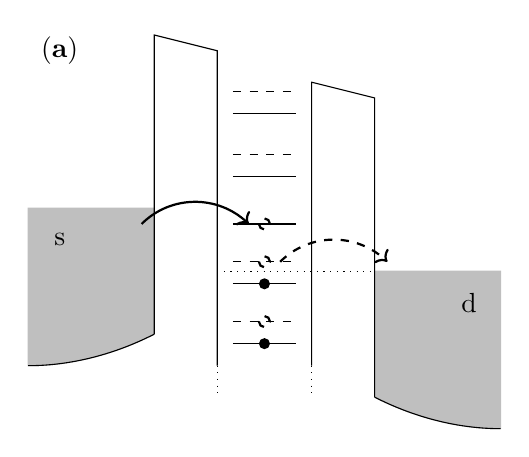
\begin{tikzpicture}[scale=0.4]
                \filldraw[color=lightgray] (0,-3) parabola (4,-2) -- (4,2) -- (0,2) -- cycle;
                \draw (0,-3) parabola (4,-2);
                \filldraw[color=lightgray] (15,-5) parabola (11,-4) -- (11,0) -- (15,0) -- cycle;
                \draw (15,-5) parabola (11,-4);
                
                \draw (4,-2) -- (4, 7.5) -- (6,7) -- (6,-3);
                \draw[dotted] (6,-3) -- (6,-4);
                
                \draw[dotted] (9,-3) -- (9,-4);
                \draw (9,-3) -- (9,6) -- (11,5.5) -- (11,-4);
                
                \draw[->,thick] (3.6,1.5) to [bend left=45] (7,1.5);
                \draw[->,thick,dashed] (8.0,0.3) to [bend left=45] (11.4,0.3);
                
                % Dot orbitals
                \draw (6.5,5) -- (8.5,5);
                \draw[dashed] (6.5,5.7) -- (8.5,5.7);
                
                \draw (6.5,3) -- (8.5,3);
                \draw[dashed] (6.5,3.7) -- (8.5,3.7);
                
                \draw[-ddot-=0.5] (6.5,1.5) -- (8.5,1.5);
                
                \draw[-dot-=0.5] (6.5,-0.4) -- (8.5,-0.4);
                \draw[-ddot-=0.5, dashed] (6.5,0.3) -- (8.5,0.3);
                
                \draw[-dot-=0.5] (6.5,-2.3) -- (8.5,-2.3);
                \draw[-ddot-=0.5, dashed] (6.5,-1.6) -- (8.5,-1.6);
                
                % Labels
                \node at (1,1) {s};
                \node at (14,-1) {d};
                
                \draw[dotted] (6,0) -- (11,0);
                \node at (1,7) {(\textbf{a})};
            \end{tikzpicture}\begin{tikzpicture}[scale=0.3]
                \draw[white] (-1,0) -- (11,0);
                \draw[->,thick] (1,8) to node[midway,above] {results in}  (9,8);
                \end{tikzpicture}
            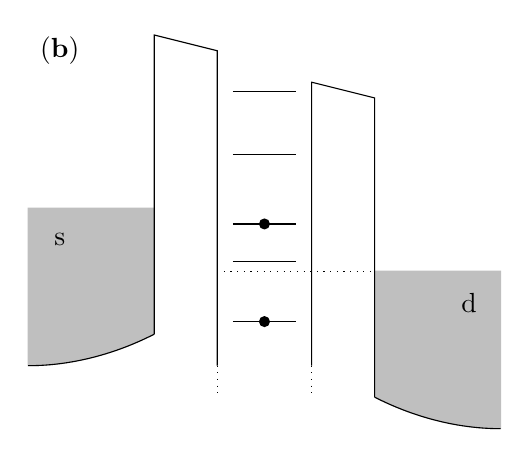
\begin{tikzpicture}[scale=0.4]
                \filldraw[color=lightgray] (0,-3) parabola (4,-2) -- (4,2) -- (0,2) -- cycle;
                \draw (0,-3) parabola (4,-2);
                \filldraw[color=lightgray] (15,-5) parabola (11,-4) -- (11,0) -- (15,0) -- cycle;
                \draw (15,-5) parabola (11,-4);
                
                \draw (4,-2) -- (4, 7.5) -- (6,7) -- (6,-3);
                \draw[dotted] (6,-3) -- (6,-4);
                
                \draw[dotted] (9,-3) -- (9,-4);
                \draw (9,-3) -- (9,6) -- (11,5.5) -- (11,-4);
                
                % Dot orbitals
                \draw (6.5,5.7) -- (8.5,5.7);
                
                \draw (6.5,3.7) -- (8.5,3.7);
                
                \draw[-dot-=0.5] (6.5,1.5) -- (8.5,1.5);
                
                \draw (6.5,0.3) -- (8.5,0.3);
                
                \draw[-dot-=0.5] (6.5,-1.6) -- (8.5,-1.6);
                
                % Labels
                \node at (1,1) {s};
                \node at (14,-1) {d};
                
                \draw[dotted] (6,0) -- (11,0);
                
                \node at (1,7) {(\textbf{b})};
            \end{tikzpicture}
        }
        \caption{Summary of tunnelling events from fig.~\ref{fig:Sequential_diagrams}. In (\textbf{a}) both tunnelling events are shown on a single diagram. Dashed lines illustrate ``the future''. Tunnelling out from the second level (shown) is just one of two possible `future' events, the other being tunnelling out from the third level, which would return the dot directly to the configuration shown in fig.~\ref{fig:Sequential_diagrams}(a). (\textbf{b}) shows the result after both tunnelling processes: a different configuration, with a different set of available tunnelling energies ($\mu$ spectrum).}
        \label{fig:Combined_diagram}
    \end{center}
    \end{figure}

    \subsection{Applicability of rate equation model}
    As discussed above, the phenomenon of Coulomb blockade can arise as a classical phenomenon, relying only on the discreteness of charge. However, the rate equation model relies on the nanocrystal having a discrete set of electron orbitals. Therefore, the theory and results of this report are not applicable to the `orthodox' classical regime, where the nanocrystal is metallic (i.e.\ has a continuous density of states). In such a situation, the theory of Averin and Likharev\cite{Averin-1991} may be used instead. %\footnote{For example, the result of rate equations shown in fig.~\ref{fig:Degeneracy}(a) diverges from the expected conductance for a \textit{metallic} nanocrystal outside the Coulomb diamonds, because it does not account for the spread of available energies in the nanocrystal.}

    \subsection{Typical parameter values}

    In experimental realisations of Coulomb blockade, often the nanocrystal is roughly spherical, is made of a metal or semiconductor, and has a diameter of a few nanometres. This typically results in single-particle energy spacings in the low hundreds of $\mathrm{meV}$\cite{Bakkers-2001}.

    Leads are usually metallic or semiconducting. One possible fabrication method is simply to let nanocrystals settle in a gap between gold electrodes\cite{Sun-2005}. Electrical contact may be aided by organic `linker' molecules\cite{Klein-1997}, which is likely to impact the source and drain capacitances. In spite of this, the classical formula for the self-capacitance of a sphere provides a very crude approximation for the total capacitance of the nanocrystal:
    \begin{equation}
        C_\mathrm{tot} \sim 4\pi\varepsilon\varepsilon_0 R
    \end{equation}
    with the relative permittivity $\varepsilon$ taken to be somewhere between its free-space value of unity and its value for (say) gold\cite{Shklyarevskii-1973} of 6.9. The resulting total capacitance is on the order of $10^{-18}\;\mathrm{F}$. In that case, the charging energy $e^2/C_\mathrm{tot}$ is also on the order of hundreds of $\mathrm{meV}$ and therefore comparable to the single-particle energy spacing.

    Many experiments have been carried out at $4.2\;\mathrm{K}$, corresponding to $k_B T = 0.36\;\mathrm{meV}$. At this temperature, the finite spread of the Fermi function is unimportant in the context of the much larger quantum mechanical and electrostatic energies.


    \section{Implementation}\label{sec:Implementation}
    The main step towards a numerical implementation of the described model of quantum Coulomb blockade is to translate equations~\ref{eqn:Rate_matrix}--\ref{eqn:Tunnel_rate_out} into code. This was carried out, to create a program that first formulates and then uses matrix equation~\ref{eqn:Rate_matrix} (or its higher-rank analogue, for more than two levels). As noted by Bonet\cite{Bonet-2002}, there are (at least) two ways to find its steady-state solution:
    \begin{description}
        \item[The eigenvalue approach:] Directly find the matrix's null vector, i.e.\ the eigenvector whose corresponding eigenvalue vanishes. Physical intuition says there should (normally) be a unique steady state and therefore a single null vector.
        \item[The evolution approach:] Evolve the weights vector under the action of the matrix in time steps, as a set of coupled differential equations, until a steady state is reached.
    \end{description}
    Whichever method is chosen, the process is carried out at each point in the configuration space -- usually points in the $\left(V_\mathrm{sd},V_\mathrm{g}\right)$ plane. At each point, once the steady state has been reached, the current (evaluated using eqn.~\ref{eqn:Current}) and weights vector are saved.

    When the simulation is run with a total of $L$ dot levels, the rate matrix has $\left(L+1\right)\times2^L$ non-zero elements, with the rest of the $2^{2L}$ elements vanishing. It is necessary to take advantage of this sparsity in order to numerically formulate and solve the system without exceeding the available \textsc{ram} in standard hardware. For $L = 16$ the number of non-zero elements is about $10^6$, and after $L$ increases past 23, memory requirements rapidly balloon into tens of gigabytes. This amounts to a strong limitation on the program's capabilities.

    Both methods were implemented and showed the same behaviour for a simple system. The eigenvalue approach was generally less robust in terms of reliably finding the null vector, and was also significantly slower, so the evolution approach was used for the bulk of the work carried out.

    The implementation uses the Runge-Kutta (RK4) method\cite{Weisstein-2015} to evolve the weights vector with time. Both step size and convergence criterion are parameters which may be varied. For simple regimes, a few hundred RK4 cycles are typically the maximum required for convergence to the steady state. Larger step sizes require fewer cycles and solve faster, but a smaller step size is often required when using more extreme parameters (e.g.\ highly asymmetric tunnel barriers, lead density of states with van~Hove singularities).

    The execution speed of the evolution approach was increased by `snaking' up and down the $\left(V_\mathrm{sd},V_\mathrm{g}\right)$ plane. Upon moving small distances in the voltage space, changes in the steady-state weights vector are small, except when crossing lines in the conductance map. Therefore, by using the previous weights vector as a guess for the new one, the new steady-state is often found in just a single iteration. In practice, plots such as those in fig.~\ref{fig:Degeneracy} with $L = 8$ can be obtained in under a minute. 

    \begin{figure}
        % Overlay "weights vector" label etc.
        \makebox[\textwidth]{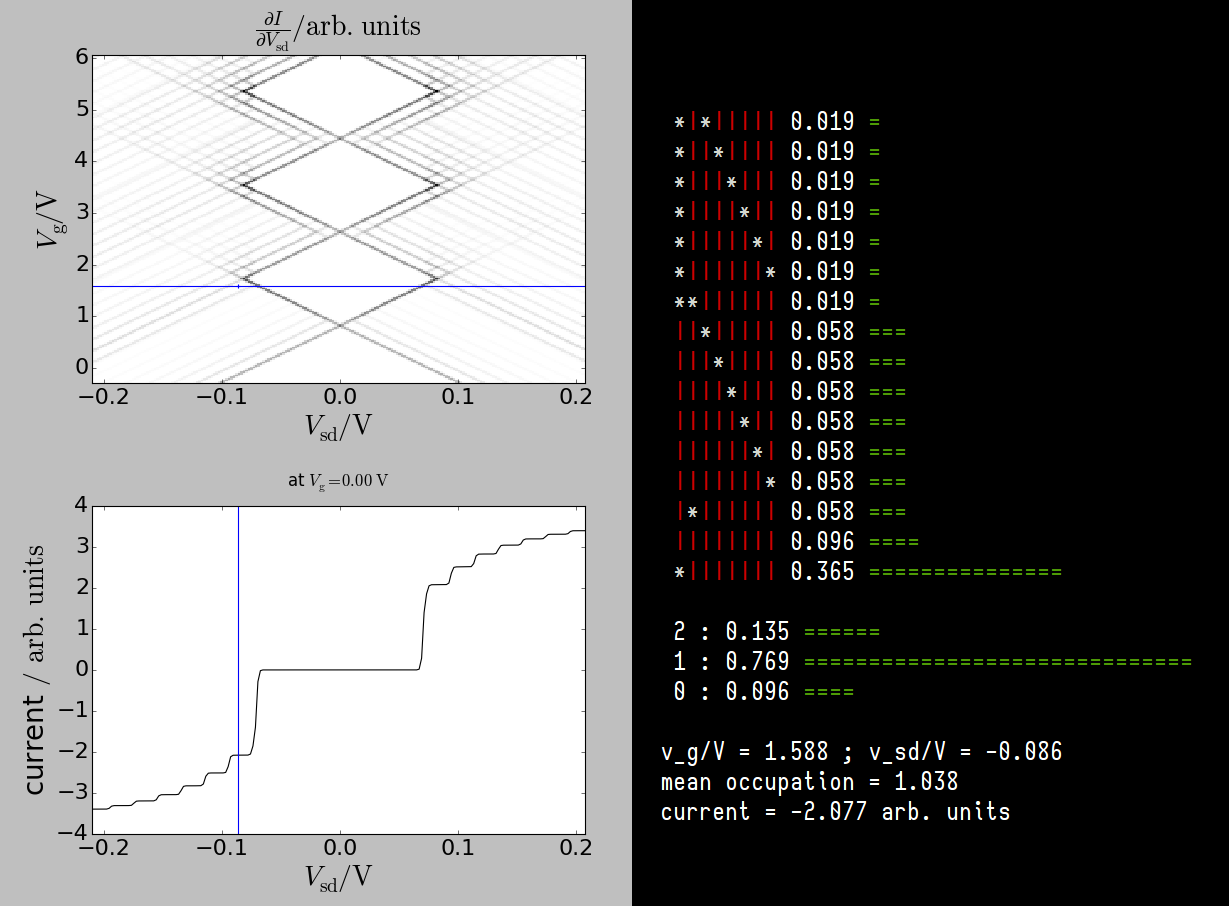
\includegraphics[scale=0.3]{img/example.png}}
        \caption{Example output of the rate equations program. The user may view the $I$--$V$ characteristic at different gate voltages, and view the weights vector at any given point in $\left(V_\mathrm{sd},V_\mathrm{g}\right)$ space. Each configuration with a non-zero weight at that point is displayed graphically as a set of unoccupied (red) and occupied (white asterisk) levels, with the lowest level leftmost. The configuration's weight is displayed alongside, as a number and a weight bar. The relative times spent with different total occupancies $N_\eta$ are also shown, below the weights vector.}
        \label{fig:Example_output}
    \end{figure}

    Sample output from the program is shown in fig.~\ref{fig:Example_output}.


    \newpage
    \section{Results and interpretation}
    Using the results from the implementation, I firstly explore the quantum mechanical-dominated regime, whose interpretation is comparatively simple. Understanding the quantum mechanical-dominated regime provides some intuition for tackling the charging-dominated regime, which comes in section~\ref{sec:Charging-dominated}. The effect of spin degeneracy and other considerations come later. A temperature of $4.2~\mathrm{K}$ and a 2-dimensional (i.e.\ flat) density of states for both source and drain leads were used except where stated.

    \subsection{Quantum mechanical-dominated regime ($\Delta E_l > e^2/C_\mathrm{tot}$)}

    Fig.~\ref{fig:QM-dominated} shows the result of a simulation for a quantum mechanical-dominated regime, with capacitances $C_\mathrm{s} = C_\mathrm{d} = 8\times10^{-18}\;\mathrm{F}$ and $C_\mathrm{g} = 8\times10^{-19}\;\mathrm{F}$ and a constant level spacing of $80\;\mathrm{meV}$. The sum of the capacitances translates to a charging energy $e^2/C_\mathrm{tot} = 9\;\mathrm{meV}$.

    \begin{figure}[h!]
    \begin{center}
        \makebox[\textwidth]{\begin{overpic}[scale=0.5]{img/qm_dominated.pdf}\put(0,0){\begin{tikzpicture}
            \draw[white] (0,0) -- (0,0.1);
            \draw[white] (10,10) -- (10,10.1);
            \draw[->,thick,magenta] (3.33,4.58) -- (4.33,3.75);
            \draw[->,thick,cyan] (3.33,4.58) -- (4.33,5.42);
            \node at (5.3,2.66) {$N = 1$};
            \node at (5.3,4.595) {$N = 2$};
            \node at (5.3,6.53) {$N = 3$};
        \end{tikzpicture}}\end{overpic}}
        \caption{Conductance map when single-particle energy exceeds charging energy. The annotated values of $N$ indicate the total occupancy number within the principal blockade diamonds. The conductance peaks encountered when moving along the magenta and cyan arrows are explained with reference to fig.~\ref{fig:QM_red-blue}.}
        \label{fig:QM-dominated}
    \end{center}
    \end{figure}

    \begin{figure}
    \begin{center}
        \makebox[\textwidth]{
            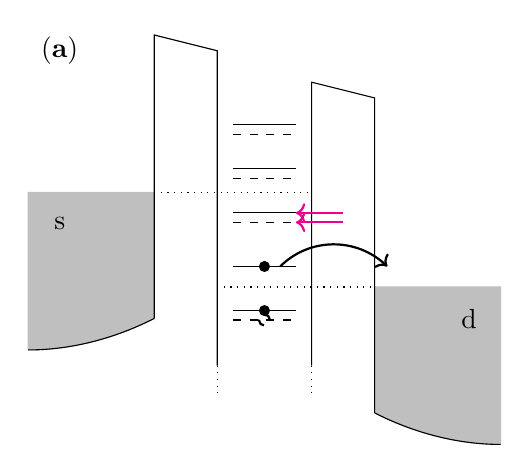
\begin{tikzpicture}[scale=0.4]
                \filldraw[color=lightgray] (0,-2.5) parabola (4,-1.5) -- (4,2.5) -- (0,2.5) -- cycle;
                \draw (0,-2.5) parabola (4,-1.5);
                \filldraw[color=lightgray] (15,-5.5) parabola (11,-4.5) -- (11,-0.5) -- (15,-0.5) -- cycle;
                \draw (15,-5.5) parabola (11,-4.5);
                
                \draw (4,-1.5) -- (4, 7.5) -- (6,7) -- (6,-3);
                \draw[dotted] (6,-3) -- (6,-4);
                
                \draw[dotted] (9,-3) -- (9,-4);
                \draw (9,-3) -- (9,6) -- (11,5.5) -- (11,-4.5);
                
                % Tunnelling
                \draw[->,thick] (8.0,0.15) to [bend left=45] (11.4,0.15);
                
                % Dot orbitals
                \draw (6.5,4.65) -- (8.5,4.65);
                \draw (6.5,3.25) -- (8.5,3.25);
                \draw (6.5,1.85) -- (8.5,1.85);
                \draw[-dot-=0.5] (6.5,0.15) -- (8.5,0.15);
                \draw[-dot-=0.5] (6.5,-1.25) -- (8.5,-1.25);
                
                % Future
                \draw[dashed] (6.5,4.35) -- (8.5,4.35);
                \draw[dashed] (6.5,2.95) -- (8.5,2.95);
                \draw[dashed] (6.5,1.55) -- (8.5,1.55);
                \draw[-ddot-=0.5,dashed] (6.5,-1.55) -- (8.5,-1.55);
                
                % Labels
                \node at (1,1.5) {s};
                \node at (14,-1.5) {d};
                
                % Guide
                \draw[dotted] (4,2.5) -- (9,2.5);
                \draw[dotted] (6,-0.5) -- (11,-0.5);
                
                \node at (1,7) {(\textbf{a})};
                
                % Red arrow
                \draw[->,thick,magenta] (10,1.85) -- (8.5,1.85);
                \draw[->,thick,magenta] (10,1.55) -- (8.5,1.55);
            \end{tikzpicture}\hspace{40pt}
            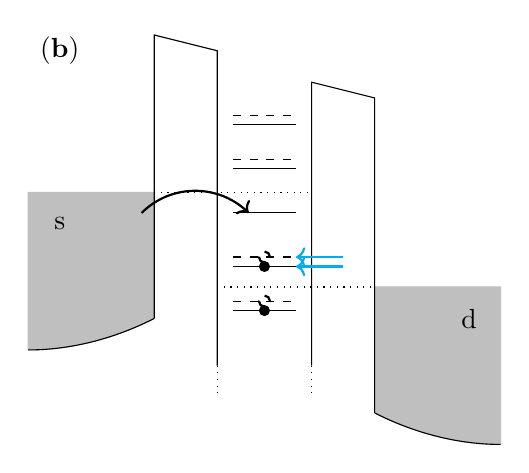
\begin{tikzpicture}[scale=0.4]
                \filldraw[color=lightgray] (0,-2.5) parabola (4,-1.5) -- (4,2.5) -- (0,2.5) -- cycle;
                \draw (0,-2.5) parabola (4,-1.5);
                \filldraw[color=lightgray] (15,-5.5) parabola (11,-4.5) -- (11,-0.5) -- (15,-0.5) -- cycle;
                \draw (15,-5.5) parabola (11,-4.5);
                
                \draw (4,-1.5) -- (4, 7.5) -- (6,7) -- (6,-3);
                \draw[dotted] (6,-3) -- (6,-4);
                
                \draw[dotted] (9,-3) -- (9,-4);
                \draw (9,-3) -- (9,6) -- (11,5.5) -- (11,-4.5);
                
                % Tunnelling
                \draw[->,thick] (3.6,1.85) to [bend left=45] (7,1.85);
                
                % Dot orbitals
                \draw (6.5,4.65) -- (8.5,4.65);
                \draw (6.5,3.25) -- (8.5,3.25);
                \draw (6.5,1.85) -- (8.5,1.85);
                \draw[-dot-=0.5] (6.5,0.15) -- (8.5,0.15);
                \draw[-dot-=0.5] (6.5,-1.25) -- (8.5,-1.25);
                
                % Future
                \draw[dashed] (6.5,4.95) -- (8.5,4.95);
                \draw[dashed] (6.5,3.55) -- (8.5,3.55);
                \draw[-ddot-=0.5,dashed] (6.5,0.45) -- (8.5,0.45);
                \draw[-ddot-=0.5,dashed] (6.5,-0.95) -- (8.5,-0.95);
                
                % Labels
                \node at (1,1.5) {s};
                \node at (14,-1.5) {d};
                
                % Guide
                \draw[dotted] (4,2.5) -- (9,2.5);
                \draw[dotted] (6,-0.5) -- (11,-0.5);
                
                \node at (1,7) {(\textbf{b})};
                
                % Red arrow
                \draw[->,thick,cyan] (10,0.45) -- (8.5,0.45);
                \draw[->,thick,cyan] (10,0.15) -- (8.5,0.15);
            \end{tikzpicture}
        }
        \caption{Energy landscape at the origin of the magenta and cyan arrows in fig.~\ref{fig:QM-dominated}, and possible tunnelling events. As before, dashed lines indicate the electrochemical potentials after a tunnelling event. The magenta- and cyan-highlighted states explain the origin of sequential conductance peaks encountered when moving through the $\left(V_\mathrm{sd},V_\mathrm{g}\right)$ plane.}
        \label{fig:QM_red-blue}
    \end{center}
    \end{figure}

    The heights of the principle diamonds are proportional to the sum of the single-particle energy spacing and the much smaller charging energy. For the $N$th Coulomb diamond, this corresponds to the spacing between the electrochemical potentials of the $N$th and $\left(N+1\right)$th levels in the configuration when only the lowest $N$ levels are occupied.

    Outside the principal diamonds, the source and drain Fermi levels do not lie in this gap, and current flows. In most regions of the $\left(V_\mathrm{sd},V_\mathrm{g}\right)$ plane, the weights vector is `flat', i.e.\ the dot spends an equal fraction of its time in each of a finite set of configurations. For instance, in the diamond where the {\color{magenta}$\searrow$}~and~{\color{cyan}$\nearrow$}~paths originate in fig.~\ref{fig:QM-dominated}, the dot spends a quarter of its time in each of the following configurations: $\{1,0,0,\dots\}$, $\{1,1,0,\dots\}$, $\{1,0,1,\dots\}$, $\{1,1,1,\dots\}$ (with all higher levels empty). This can be understood with reference to fig.~\ref{fig:QM_red-blue}. The individual tunnel rates are all equal as a consequence of the (flat) lead densities-of-states (and tunnel width invariance) and furthermore, the statistics of tunnelling are independent of which of the accessible configurations the dot happens to be in at a given moment. We could say that the two single-particle states are `orthogonal' in a sense, or act as separate electrical systems in parallel.

    Moving along either of the {\color{magenta}$\searrow$}, {\color{cyan}$\nearrow$}~paths (i.e.\ varying either the source or drain Fermi level) leads to a breakdown of this orthogonality in a narrow region of the $\left(V_\mathrm{sd},V_\mathrm{g}\right)$ plane. Between the two conductance peaks on the {\color{magenta}$\searrow$} path, the electrochemical potential of the upper accessible level falls below the source Fermi level if and only if the lower level is empty (fig.~\ref{fig:QM_red-blue}(a)). As a consequence, the weights of the four accessible configurations are as follows:
    \begin{align*}
        w{\left(\{1,1,0,\dots\}\right)} = 43.8\;\%,\\
        w{\left(\{1,0,0,\dots\}\right)} = 31.3\;\%,\\
        w{\left(\{1,0,1,\dots\}\right)} = 18.7\;\%,\\
        w{\left(\{1,1,1,\dots\}\right)} = {\color{white}0}6.2\;\%.
    \end{align*}

    As the difference between source and drain Fermi levels increases to span $N$ dot levels, the number of possible total occupancies increases to $N$, and with it the number of possible total electrostatic energy values. This is the reason for the increasing number of parallel lines surrounding the diamonds at higher source-drain bias.

    \subsection{Charging-dominated regime ($\Delta E_l < e^2/C_\mathrm{tot}$)}\label{sec:Charging-dominated}

    In the charging-dominated regime, the large charging energy means that vacant levels have their electrochemical potentials shifted a large distance up from occupied ones. When source and drain Fermi levels lie in the gap between occupied and unoccupied levels, the dot undergoes conventional Coulomb blockade. This is responsible for the principal diamonds in fig.~\ref{fig:Zoom}(a). If the gate voltage is altered such that the lead Fermi levels no longer lie in the gap, the blockade is lifted, as shown in fig.~\ref{fig:Current_flow}.

    \begin{figure}[h!]
    \begin{center}
        \makebox[\textwidth]{
            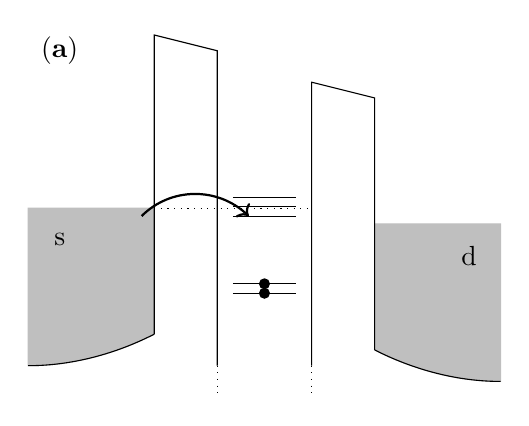
\begin{tikzpicture}[scale=0.4]
                \filldraw[color=lightgray] (0,-3) parabola (4,-2) -- (4,2) -- (0,2) -- cycle;  % Source Fermi level
                \draw (0,-3) parabola (4,-2);
                
                \filldraw[color=lightgray] (15,-3.5) parabola (11,-2.5) -- (11,1.5) -- (15,1.5) -- cycle;  % Drain Fermi level
                \draw (15,-3.5) parabola (11,-2.5);
                
                % Barriers
                \draw (4,-2) -- (4, 7.5) -- (6,7) -- (6,-3);
                \draw[dotted] (6,-3) -- (6,-4);
                \draw[dotted] (9,-3) -- (9,-4);
                \draw (9,-3) -- (9,6) -- (11,5.5) -- (11,-2.5);
                
                % Tunnelling
                \draw[->,thick] (3.6,1.75) to [bend left=45] (7,1.75);
                
                % Guide
                \draw[dotted] (4,2) -- (9,2);
                
                % Dot orbitals
                
                \draw (6.5,2.35) -- (8.5,2.35);
                \draw (6.5,2.05) -- (8.5,2.05);
                \draw (6.5,1.75) -- (8.5,1.75);
                
                \draw[-dot-=0.5] (6.5,-0.4) -- (8.5,-0.4);
                \draw[-dot-=0.5] (6.5,-0.7) -- (8.5,-0.7);
                
                % Labels
                \node at (1,1) {s};
                \node at (14,0.5) {d};
                
                \node at (1,7) {(\textbf{a})};
            \end{tikzpicture}\begin{tikzpicture}[scale=0.3]
                \draw[white] (-1,0) -- (11,0);
                \draw[->,thick] (1,9) to [bend left=30]  (9,9);
                \draw[->,thick] (9,7) to [bend left=30]  (1,7);
                \node at (5,8) {cycle};
                \end{tikzpicture}
            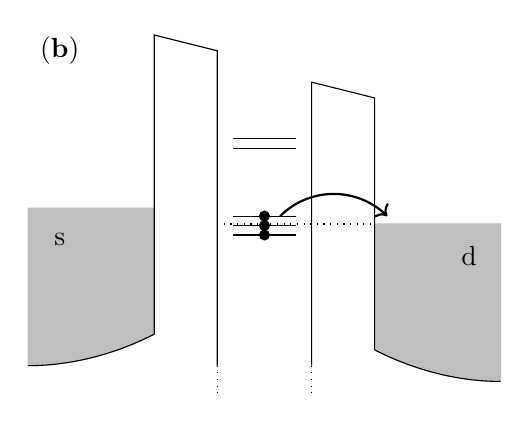
\begin{tikzpicture}[scale=0.4]
                \filldraw[color=lightgray] (0,-3) parabola (4,-2) -- (4,2) -- (0,2) -- cycle;  % Source Fermi level
                \draw (0,-3) parabola (4,-2);
                
                \filldraw[color=lightgray] (15,-3.5) parabola (11,-2.5) -- (11,1.5) -- (15,1.5) -- cycle;  % Drain Fermi level
                \draw (15,-3.5) parabola (11,-2.5);
                
                % Barriers
                \draw (4,-2) -- (4, 7.5) -- (6,7) -- (6,-3);
                \draw[dotted] (6,-3) -- (6,-4);
                \draw[dotted] (9,-3) -- (9,-4);
                \draw (9,-3) -- (9,6) -- (11,5.5) -- (11,-2.5);
                
                % Dot orbitals
                \draw (6.5,4.20) -- (8.5,4.20);
                \draw (6.5,3.9) -- (8.5,3.9);
                \draw[-dot-=0.5] (6.5,1.75) -- (8.5,1.75);
                \draw[-dot-=0.5] (6.5,1.45) -- (8.5,1.45);
                \draw[-dot-=0.5] (6.5,1.15) -- (8.5,1.15);
                
                \draw[->,thick] (8.0,1.75) to [bend left=45] (11.4,1.75);
                
                % Guide
                \draw[dotted] (6,1.5) -- (11,1.5);
                
                % Labels
                \node at (1,1) {s};
                \node at (14,0.5) {d};
                
                \node at (1,7) {(\textbf{b})};
            \end{tikzpicture}
        }
        \caption{Simplest possible current flow in the charging-dominated regime. This cycle can occur near the vertex between the $N = 2$ and $N = 3$ diamonds. Only the lowest five dot levels are shown.}
        \label{fig:Current_flow}
    \end{center}
    \end{figure}

    Fig.~\ref{fig:Zoom} shows the result of a simulation with $C_\mathrm{s} = C_\mathrm{d} = 1\times10^{-18}\;\mathrm{F}$ and $C_\mathrm{g} = 1\times10^{-19}\;\mathrm{F}$ and a constant level spacing of $10\;\mathrm{meV}$, with 8 levels total. The sum of the capacitances translates to a charging energy $e^2/C_\mathrm{tot} = 73\;\mathrm{meV}$.

    \begin{figure}[p]
    \begin{center}
        \makebox[\textwidth]{
            \begin{overpic}[scale=0.4]{img/broken_degeneracy.pdf}
                \put(0,0){\begin{tikzpicture}[scale=0.9]
                    \draw[white] (0,0) -- (0.2,0.2);
                    \draw[dotted,thick] (2.8,2) -- (2.8,4.3) -- (4.9,4.3) -- (4.9,2) -- cycle;
                    %\draw (2.45,2.15) -- (1.2,2.8);
                    %\draw (2.45,3.45) -- (1.2,4.1);
                    %\draw (2.45,4.75) -- (1.2,5.4);
                    \node at (0.2,7) {(\textbf{a})};
                \end{tikzpicture}}
            \end{overpic}
            \begin{overpic}[scale=0.4,trim=0 25pt 0 0]{img/zoom.pdf}
                \put(0,0){\begin{tikzpicture}
                    \draw[white] (0,0) -- (0.2,0.2);
                    \node at (0.2,8.1) {(\textbf{b})};
                    \draw[->,thick,magenta] (1.55,2.55) -- (2.6,2.05);
                \end{tikzpicture}}
            \end{overpic}
        }
        \caption{Charge stability map when charging energy exceeds single-particle energy spacing. (\textbf{a}) shows the first three Coulomb blockade diamonds, with excitation spectra outside. (\textbf{b}) shows detail of the inset region, with annotated paths, features of which are explained in later figures.}
        \label{fig:Zoom}
    \end{center}
    \end{figure}

    \begin{figure}[p]
    \begin{center}
        \makebox[\textwidth]{\begin{overpic}[scale=0.4]{img/iv_blockade.pdf}\put(5,73){(\textbf{a})}\end{overpic}\begin{overpic}[scale=0.4]{img/iv.pdf}\put(5,73){(\textbf{b})}\end{overpic}}
        \caption{$I$--$V$ curves at different gate voltages in the charging-dominated regime. (\textbf{a}) shows Coulomb blockade and (\textbf{b}) shows a position where it has been lifted by applying a different gate voltage. (\textbf{a}) shows decreasing marginal current increase as more of the excitation spectra becomes available for tunnelling.}
        \label{fig:IV_curve}
    \end{center}
    \end{figure}

    Each blockade diamond comes with an associated excitation spectrum existing outside the diamond. For the $N$th blockade diamond, there are $N-1$ excitation lines parallel to its lower edges and $L - N - 1$ excitation lines parallel to its upper edge, where $L$ is the total number of levels in the dot. These conductance lines can be interpreted as the sequential `turning-on' of tunnelling through the extra levels illustrated in fig.~\ref{fig:Current_flow}, as source Fermi level is increased or drain Fermi level decreased. Part of the excitation spectrum running parallel to the top edge of each diamond also protrudes below the diamond corner (see magenta path in fig.~\ref{fig:Zoom}(b)). This has a more subtle origin, elucidated by fig.~\ref{fig:Strange-line}.

    In contrast to the quantum mechanical-dominated case, the conducting states in this regime cannot be treated as separate electrical systems in parallel. This is demonstrated by the reduction in marginal current increase as successive levels in the excitation spectrum become available (e.g.\ fig.~\ref{fig:IV_curve}(a)). This phenomenon may seem counter-intuitive, as the rate of tunnelling in ought to be proportional to the number of available levels to tunnel into. However, tunnelling in to any one of the available levels raises all other levels above the source Fermi energy, so the net current flow is limited by the rate of tunnelling out. This fact explains the `levelling-off' of current with increasing source-drain bias.

    \begin{figure}
    \begin{center}
        \makebox[\textwidth]{
            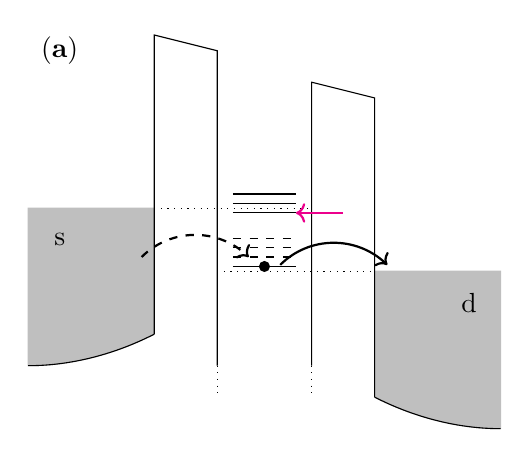
\begin{tikzpicture}[scale=0.4]
                \filldraw[color=lightgray] (0,-3) parabola (4,-2) -- (4,2) -- (0,2) -- cycle;
                \draw (0,-3) parabola (4,-2);
                \filldraw[color=lightgray] (15,-5) parabola (11,-4) -- (11,0) -- (15,0) -- cycle;
                \draw (15,-5) parabola (11,-4);
                
                \draw (4,-2) -- (4, 7.5) -- (6,7) -- (6,-3);
                \draw[dotted] (6,-3) -- (6,-4);
                
                \draw[dotted] (9,-3) -- (9,-4);
                \draw (9,-3) -- (9,6) -- (11,5.5) -- (11,-4);
                
                % Tunnelling
                \draw[->,thick] (8.0,0.2) to [bend left=45] (11.4,0.2);
                
                % Dot orbitals
                \draw (6.5,2.45) -- (8.5,2.45);
                \draw (6.5,2.15) -- (8.5,2.15);
                \draw (6.5,1.85) -- (8.5,1.85);
                \draw[-dot-=0.5] (6.5,0.15) -- (8.5,0.15);
                % \draw[-dot-=0.5] (6.5,-0.-0.15) -- (8.5,-0.15);
                
                % Future
                \draw[dashed] (6.5,1.05) -- (8.5,1.05);
                \draw[dashed] (6.5,0.75) -- (8.5,0.75);
                \draw[dashed] (6.5,0.45) -- (8.5,0.45);
                % \draw[-ddot-=0.5,dashed] (6.5,-1.45) -- (8.5,-1.45);
                
                % Future tunnelling
                \draw[->,thick,dashed] (3.6,0.45) to [bend left=45] (7,0.45);
                
                % Labels
                \node at (1,1) {s};
                \node at (14,-1) {d};
                
                % Guide
                \draw[dotted] (4,2) -- (9,2);
                \draw[dotted] (6,0) -- (11,0);
                
                \node at (1,7) {(\textbf{a})};
                
                % Red arrow
                \draw[->,thick,magenta] (10,1.85) -- (8.5,1.85);
            \end{tikzpicture}\begin{tikzpicture}[scale=0.3]
                \draw[white] (-1,0) -- (11,0);
                \draw[->,thick] (1,8) to node[midway,above] {results in}  (9,8);
                \end{tikzpicture}
            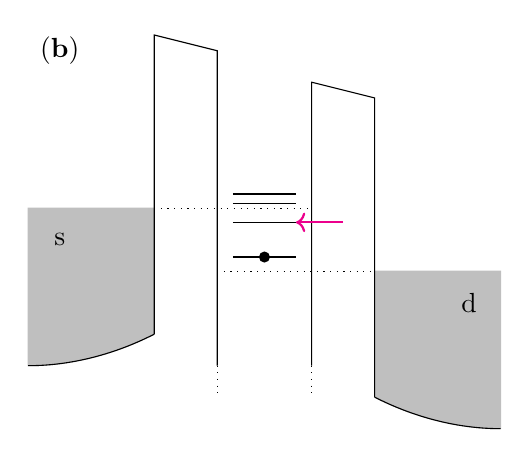
\begin{tikzpicture}[scale=0.4]
                \filldraw[color=lightgray] (0,-3) parabola (4,-2) -- (4,2) -- (0,2) -- cycle;
                \draw (0,-3) parabola (4,-2);
                \filldraw[color=lightgray] (15,-5) parabola (11,-4) -- (11,0) -- (15,0) -- cycle;
                \draw (15,-5) parabola (11,-4);
                
                \draw (4,-2) -- (4, 7.5) -- (6,7) -- (6,-3);
                \draw[dotted] (6,-3) -- (6,-4);
                
                \draw[dotted] (9,-3) -- (9,-4);
                \draw (9,-3) -- (9,6) -- (11,5.5) -- (11,-4);
                
                % Dot orbitals
                \draw (6.5,2.45) -- (8.5,2.45);
                \draw (6.5,2.15) -- (8.5,2.15);
                \draw (6.5,1.55) -- (8.5,1.55);
                \draw[-dot-=0.5] (6.5,0.45) -- (8.5,0.45);
                % \draw[-dot-=0.5] (6.5,-0.-0.15) -- (8.5,-0.15);
                
                % Labels
                \node at (1,1) {s};
                \node at (14,-1) {d};
                
                % Guide
                \draw[dotted] (4,2) -- (9,2);
                \draw[dotted] (6,0) -- (11,0);
                
                \node at (1,7) {(\textbf{b})};
                
                % Red arrow
                \draw[->,thick,magenta] (10,1.55) -- (8.5,1.55);
            \end{tikzpicture}
        }
        \caption{Physical origin of conductance peaks near diamond edges in the charging-dominated regime. (\textbf{a}) shows a possible sequence of tunnelling events, leading to (\textbf{b}). Moving along the {\color{magenta}$\searrow$} path in fig.~\ref{fig:Zoom} path lowers the source Fermi level with respect to the dot levels (see fig.~\ref{fig:Directions} for a reminder). The fall of the source Fermi level firstly below the magenta highlighted potential in (\textbf{a}), and then that in (\textbf{b}), is responsible for the sequential conductance peaks encountered when traversing this path. For clarity, only the lowest four dot orbitals are shown.}
        \label{fig:Strange-line}
    \end{center}
    \end{figure}

    %If a simulation with a larger number of dot levels was run, the excitation spectra would continue indefinitely moving outwards and upwards in $\left(V_\mathrm{sd},V_\mathrm{g}\right)$ space. Although their effect falls monotonically as more of the excitation spectrum becomes available for tunnelling, this means that the program, limited to a small number of dot levels, only accurately predicts the conductance map in regions close to the principal blockade diamonds.

    \newpage
    \subsection{Spin degeneracy}

    \begin{figure}
    \begin{center}
        \makebox[\textwidth]{\begin{overpic}[scale=0.4]{img/qm_dominated_spin.pdf}\put(5,73){(\textbf{a})}\end{overpic}\begin{overpic}[scale=0.4]{img/broken_degeneracy_spin.pdf}\put(5,73){(\textbf{b})}\end{overpic}}
        \caption{Effect of spin degeneracy in (\textbf{a}) quantum mechanical-dominated regime and (\textbf{b}) charging-dominated regime. In the latter, the excitation spectra occupy less of the plot compared to the spinless plot (fig.~\ref{fig:Zoom}) because a truncated single-particle spectrum was used.}
        \label{fig:Spin_degenaracy}
    \end{center}
    \end{figure}

    In the rate equation model, spin degeneracy can be incorporated simply by using pairs of levels with equal single-particle energies. Fig.~\ref{fig:Spin_degenaracy} shows the result of doing this. In the quantum mechanical-dominated regime, the effect is to map every line in the old, spinless conductance map (fig.~\ref{fig:QM-dominated}) to a pair of lines in the new one, offset vertically by an amount proportional to the charging energy.

    In the charging-dominated regime, spin degeneracy modifies certain features of the excitation spectra, and sharpens the edges of the even-numbered diamonds, compared to the spinless behaviour in fig.~\ref{fig:Zoom}. By way of explanation, consider the lower edge of the second Coulomb diamond in fig.~\ref{fig:Spin_degenaracy}. Here, tunnelling in to one of the lowest pair of level raises the potential of the other, occupied, level so that tunnelling out may occur from either level, doubling the tunnelling-out rate and thereby increasing the current compared to the spinless case. Something resembling this sharpened conductance in alternating diamonds has been observed experimentally\cite{Larsson-2011}.

    \begin{figure}[h]
    \begin{center}
        \makebox[\textwidth]{\begin{overpic}[scale=0.4]{img/asymmetry.pdf}\put(5,73){(\textbf{a})}\end{overpic}\begin{overpic}[scale=0.4]{img/van_hove.pdf}\put(5,73){(\textbf{b})}\end{overpic}}
        \caption{Effect on the conductance map of (\textbf{a}) source-drain asymmetry and (\textbf{b}) a van~Hove singularity in the lead densities-of-states. In (\textbf{b}) the grey which dominates the plot indicates zero conductance and lighter shades show negative conductance.}
        \label{fig:Asymmetry}
    \end{center}
    \end{figure}

    \newpage
    \subsection{Mixed regime, lead asymmetry and van~Hove singularities}

    Most experiments are carried out in a regime where the single-particle energy spacings and the charging energy are quite similar. Fig.~\ref{fig:Asymmetry} shows a simulation carried out in this regime, with spin degeneracy as well as other complicating factors included.

    In experiments using nanocrystals, there is often asymmetry between the source and drain leads. This can take two forms: tunnel rate asymmetry and capacitance asymmetry. Fig.~\ref{fig:Asymmetry}(a) demonstrates both effects. Slight geometric skewing of the diamonds is the main consequence of capacitance asymmetry, while tunnel rate asymmetry (in this case weaker source-dot coupling than dot-drain) results in the increased prevalence of positively-sloped lines in the conductance map. In general, tunnel rates are expected to fall off exponentially with dot-lead separation, while capacitance variation is only polynomial, so tunnel rate asymmetry is expected to be a more important effect.

    Experimenters who used two-dimensional leads\cite{Fuechsle-2010} reported that finely-spaced lines (conductance peaks) outside the blockade diamonds were caused by van~Hove singularities in the lead densities of states. Fig.~\ref{fig:Asymmetry}(b) shows that the rate equation approach can account for this phenomenon. To produce this plot I included a single van~Hove singularity, $10\;\mathrm{meV}$ below the lead Fermi energies. Such singularities make for much slower program execution, with thousands of iterations often required to find steady states.

    \subsection{Band gap in leads}
    \begin{figure}
    \begin{center}
        \makebox[\textwidth]{\begin{overpic}[scale=0.4]{img/small_band_gap.pdf}\put(5,73){(\textbf{a})}\end{overpic}\hspace{10pt}
        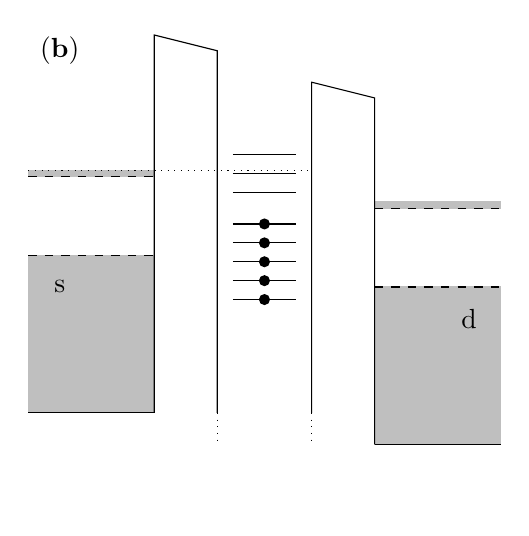
\begin{tikzpicture}[scale=0.4]
            \filldraw[color=lightgray] (0,-4.5) -- (4,-4.5) -- (4,0.5) -- (0,0.5) -- cycle;
            \filldraw[lightgray] (0,3) -- (4,3) -- (4,3.2) -- (0,3.2) -- cycle;
            \draw (0,-4.5) -- (4,-4.5);
            \filldraw[color=lightgray] (15,-5.5) -- (11,-5.5) -- (11,-0.5) -- (15,-0.5) -- cycle;
            \filldraw[lightgray] (11,2) -- (15,2) -- (15,2.2) -- (11,2.2) -- cycle;
            \draw (15,-5.5) -- (11,-5.5);
            
            \draw[dashed] (0,0.5) -- (4,0.5);
            \draw[dashed] (0,3) -- (4,3);
            \draw[dotted] (0,3.2) -- (9,3.2);
            
            \draw[dashed] (11,-0.5) -- (15,-0.5);
            \draw[dashed] (11,2) -- (15,2);
            
            \draw (4,-4.5) -- (4, 7.5) -- (6,7) -- (6,-4.5);
            \draw[dotted] (6,-4.5) -- (6,-5.5);
            
            \draw[dotted] (9,-4.5) -- (9,-5.5);
            \draw (9,-4.5) -- (9,6) -- (11,5.5) -- (11,-5.5);
            
            % Tunnelling
            %\draw[->,thick] (8.0,0.15) to [bend left=45] (11.4,0.15);
            
            % Dot orbitals
            \draw (6.5,3.7) -- (8.5,3.7);
            \draw (6.5,3.1) -- (8.5,3.1);
            \draw (6.5,2.5) -- (8.5,2.5);
            \draw[-dot-=0.5] (6.5,1.5) -- (8.5,1.5);
            \draw[-dot-=0.5] (6.5,0.9) -- (8.5,0.9);
            \draw[-dot-=0.5] (6.5,0.3) -- (8.5,0.3);
            \draw[-dot-=0.5] (6.5,-0.3) -- (8.5,-0.3);
            \draw[-dot-=0.5] (6.5,-0.9) -- (8.5,-0.9);
            
            % Labels
            \node at (1,-0.5) {s};
            \node at (14,-1.5) {d};
            
            % Guide
            %\draw[dotted] (4,2.5) -- (9,2.5);
            %\draw[dotted] (6,-0.5) -- (11,-0.5);
            
            \draw[white] (0,-7.5) -- (1,-7.5);
            \node at (1,7) {(\textbf{b})};
        \end{tikzpicture}\hspace{20pt}
        }
        \caption{Addition of an unrealistically small ($70\;\mathrm{meV}$) band gap in the leads, with the Fermi level lying just above the conduction band edge (i.e.\ n-doping). (\textbf{a}) shows the effect on the conductance map, with grey in most areas representing zero conductance and white showing negative conductance. (\textbf{b}) shows a possible dot configuration between leads with a band gap.}
        \label{fig:Band_gap}
    \end{center}
    \end{figure}

    Fig.~\ref{fig:Band_gap}(a) shows the effect of adding a small band gap to the lead densities-of-states, in the mixed regime previously used in fig.~\ref{fig:Asymmetry}(a). A more realistic simulation would have many more levels lying in the band gap, but this is difficult to achieve computationally because of the limit on the number of levels usable in the rate equation implementation.

    Despite the unrealistic nature of the parameters used, three main features of the conductance map are worthy of comment. Firstly, the lower edges of the principal blockade diamonds are removed completely. Secondly, the band gap introduces negative conductance immediately outside those parts of the principal blockade diamonds which remain. Thirdly, there is a consistent current flow once the source-drain bias exceeds the band gap. Each of these observations are physically reasonable and explainable in terms of chemical potential diagrams, but the conductance map does not resemble anything seen in the literature.

    %\newpage
    \section{Outlook}

    Conductance maps calculated using the rate equation approach, such as fig.~\ref{fig:Asymmetry}, bear a good resemblance to experimentally realised plots, in e.g.\ \oldcite{Kouwenhoven-1997}, \oldcite{Dushmukh-2002}, \oldcite{Fuechsle-2010}. However, there are a number of areas in the implementation which could be improved.

    The constant interaction assumption could be relaxed quite simply within the model, by altering the form of the electrochemical potentials (eqn.~\ref{eqn:Chemical_potential}) to depend on the full form of the configuration $\eta$, rather than simply the total occupancy $N_\eta$.

    Thus far, the source and drain tunnel rates were assumed to be constant for a given level. In reality the tunnel rates are likely to depend on the applied bias and the electrochemical potential of the level. If incorporated into the model, these effects might alter the sharpness of different lines in the conductance map.

    The effect of relaxation could be included by incorporating the relevant matrix elements in eqn.~\ref{eqn:Rate_matrix}. This would, however, significantly increase the number of matrix elements and slow down the simulation as a consequence.

    Cotunnelling is an important feature of some experimentally realised conductance maps\cite{Guttinger-2012}, where blockade is broken within the principal diamonds, by the coherent motion of two electrons. It seems that the rate equation approach I have used cannot incorporate this sort of behaviour, and other methods, which account for coherence, would be required.

    Within the rate equation approach, it may be possible to use certain equivalences about tunnelling rates for different levels to reduce the number of matrix elements required and thus speed up execution for many-level systems\cite{Klimeck-1994}. However, I do not think this can be achieved whilst retaining generality about the baseline tunnelling rates and the lead densities-of-states.

    % bias itself might increase the distance over which the electron must tunnel (see e.g.\ Deshpande 2000 fig~3) $\implies$ asymmetry considerations

    % As discussed, it seems as though flow should be quite sensitive to the exact nature of the contact between dot and electrode. To date, in most other simulations of this type, the effect of lead densities-of-states seems not to have been addressed. Therefore, need to understand whether the bulk band structure is the right thing to use, and what effect, if any, linker molecules have.


    \section{Conclusion}
    A model of transport through a quantum dot was introduced, based on rate equations, constant interaction and Fermi's golden rule. The model was implemented numerically using both eigenvalue and \textsc{ode} methods, which both produced the same results. The faster \textsc{ode} method was used to investigate and account for current characteristics in two main regimes: quantum mechanical-dominated and electrostatically-dominated. The effects of spin degeneracy, source-drain asymmetry and singularities in lead densities-of-states were studied, and the results were found to be largely consistent with experimental observations. The model was applied tentatively to the case of n-doped semiconducting leads, and it was noted that further work is required to generate reliable results in this regime. Finally, suggestions were made about possible ways to improve the implementation, including relaxing the assumption of constant interaction and incorporating electronic relaxation.

    \newpage
    \addcontentsline{toc}{section}{References}
    \bibliographystyle{plain}
    \bibliography{all}

    \newpage
    \appendix
    \section{Appendix}
    \subsection{Derivation of electrochemical potential}\label{sec:Chemical_potential}
    In the constant interaction model, the total energy for a configuration is the sum of its single-particle energies plus the electrostatic energy $Q^2/2C$. Therefore:
    \begin{align*}
        \mu_{l|\eta}^+ =\; &E_{\eta^\prime} - E_{\eta} \\
        =\; &E_l + \frac{\left[\left(N_{\eta}+1\right)\left(-e\right) + \sum\nolimits_i C_i V_i\right]^2}{2\sum\nolimits_i C_i} - \frac{\left[N_{\eta}\left(-e\right) + \sum\nolimits_i C_i V_i\right]^2}{2\sum\nolimits_i C_i} \\
        =\; &E_l + \frac{1}{2\sum\nolimits_i C_i}\left[\left(N_{\eta}^2 + 2N_{\eta} + 1\right)e^2 - 2 \left(N_{\eta} + 1\right)e\sum_i C_i V_i + \left(\sum_i C_i V_i\right)^2\right] + \\
        &\;\;\;\;- \frac{1}{2\sum\nolimits_i C_i}\left[N_{\eta}^2 e^2 - 2 N_{\eta} e\sum_i C_i V_i + \left(\sum_i C_i V_i\right)^2\right] \\
        =\; &E_l + \frac{e}{\sum\nolimits_i C_i}\left[\left(N_{\eta} + \frac{1}{2}\right)e - \sum_i C_i V_i\right].
    \end{align*}
    For $\mu_{l|\eta}^-$ we make the replace $N_{\eta}$ with $\left(N_{\eta} - 1\right)$ so
    \begin{align*}
        \mu_{l|\eta}^- =\; &E_l + \frac{e}{\sum\nolimits_i C_i}\left[\left(N_{\eta} - \frac{1}{2}\right)e - \sum_i C_i V_i\right].
    \end{align*}

\end{document}
